\documentclass{article}
\usepackage{amsmath, amssymb, tikz, geometry, graphicx, natbib, mwe, color, xcolor, listings, tabularx, pdfpages, blindtext, mathtools, stackengine, pgfplots,bigints, relsize, upgreek, esint, array, multirow, schemata, wrapfig, cancel, comment}
\usepackage{hyperref}
\usepackage{slashed, enumitem}
\usepackage{titlesec}
\usetikzlibrary{positioning}

\begin{comment}
code to write section, subsection and subsubsection title in a specific color
\titleformat{\section}
{\color{synthwave_text}\normalfont\Large\bfseries}
{\color{synthwave_text}\thesection}{1em}{} 

\titleformat{\subsection}
{\color{synthwave_text}\normalfont\large\bfseries}
{\color{synthwave_text}\thesubsection}{1em}{} 

\titleformat{\subsubsection}
{\color{synthwave_text}\normalfont\normalfont\bfseries}
{\color{synthwave_text}\thesubsubsection}{1em}{}
\end{comment}


\pgfplotsset{compat=1.9}

\colorlet{myWhite}{white!35!gray}
\definecolor{shadeofgray}{HTML}{181818}
\definecolor{shadeofviolet}{HTML}{0f022c}
\definecolor{synthwave_beckground}{HTML}{252334}
\definecolor{synthwave_text}{HTML}{e148aa}


\hypersetup{
    colorlinks=true,
    linkcolor=violet,
    filecolor=magenta,      
    urlcolor=cyan,
    pdftitle={Controlli Automatici T},
    pdfpagemode=FullScreen,
}


\geometry{ 
 a4paper,
 left=10mm,
 right=10mm,
 top=10mm
 }
 
\lstdefinestyle{mystyle}{ 
bracketsstyle=\color{red}
}

\title{Controlli Automatici T}
\author{Giuseppe Bumma}


% color option
%\pagecolor{synthwave_beckground} %{shadeofgray}
%\color{myWhite}

\renewcommand{\CancelColor}{\color{synthwave_text}}


\begin{document}

%Commands
\newcommand{\R}{\mathbb{R}}
\newcommand{\Varepsilon}{\mathcal{E}}
\newcommand{\rad}{\text{rad}}
\newcommand{\bb}[1]{\mathbb{#1}}
\newcommand{\cc}[1]{\mathcal{#1}}
\newcommand{ \lognormal }{\text{Lognormal} }
\newcommand{\T}[1]{\text{#1}}
\newcommand*\circled[1]{\tikz[baseline=(char.base)]{%
            \node[shape=circle,draw,inner sep=2pt] (char) {#1};}}
%for using circled number in enumerate use:
%\begin{enumerate}[label=\protect\circled{\arabic*}]


\tableofcontents

\maketitle

\section{Introduzione}
L'idea dei \textbf{controlli automatici} è sostituire l'intelligenza umana con un sistema automatico (come l'intelligenza artificiale) basata su leggi matematiche e/o algoritmi.



\subsection{Notazione ed elementi costitutivi}
\begin{center}
    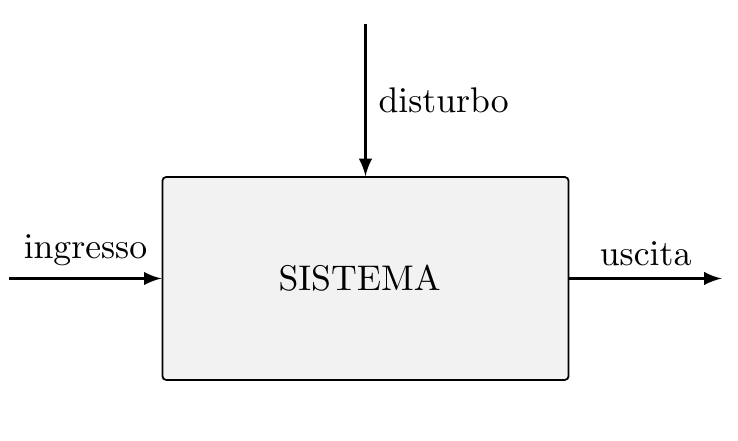
\includegraphics[scale=0.3]{Images/Schema_sistema.png}
\end{center}
Il \textbf{sistema} è un oggetto per il quale si vuole ottenere un comportamento desiderato.
\\
Esempi di sistema sono: impianto (industriale), macchinario (braccio robotico, macchina a controllo numerico, etc\dots), veicolo (auto, velivolo, drone, etc\dots), fenomeno fisico (condizioni atmosferiche), sistema biologico, sistema sociale.
\\
L'obiettivo è che l'andamento nel tempo di alcune variabili segua un segnale di riferimento.
\vspace*{0.2cm}\\
Altri elementi sono:
\begin{itemize}
    \item Controllore: unità che determina l'andamento della variabile di controllo (ingresso);
    \item Sistema di controllo: sistema (processo) + controllore;
    \item Sistemi di controllo naturali: meccanismi presenti in natura, come  quelli presenti nel corpo umano (temperatura corporea costante, ritmo cardiaco, etc\dots);
    \item Sistemi di controllo manuali: è presente l'azione dell'uomo;
    \item Sistemi di controllo automatico: uomo sostituito da un dispositivo.
\end{itemize}




\subsection{Controllo in anello aperto e anello chiuso}
Controllo in anello aperto (“feedforward”): il controllore utilizza solo il segnale di riferimento
\begin{center}
    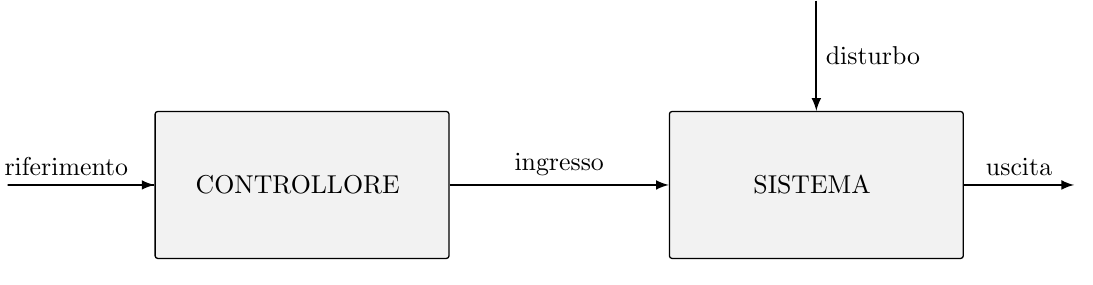
\includegraphics[scale=0.32]{Images/Anello_aperto.png}
\end{center}
Controllo in anello chiuso (“feedback” o retroazione): il controllore utilizza il segnale di riferimento e la variabile controllata ad ogni istante di tempo
\begin{center}
    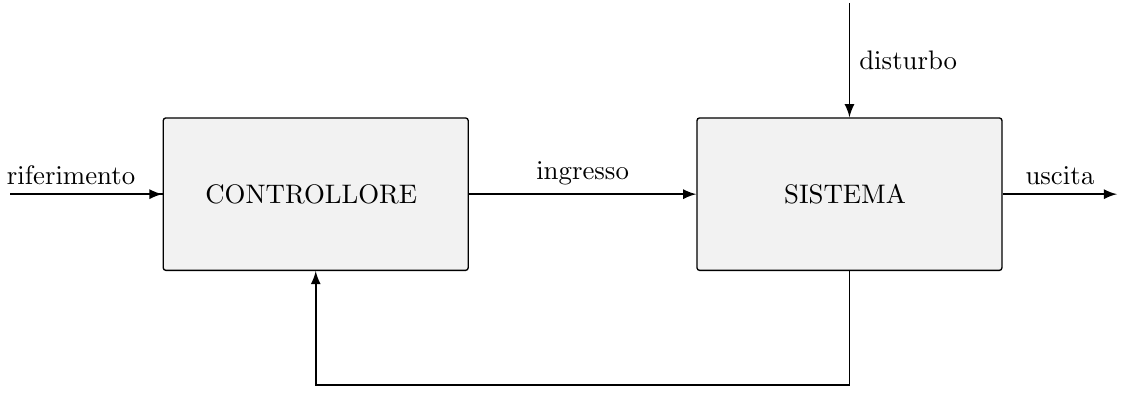
\includegraphics[scale=0.3]{Images/Anello_chiuso.png}
\end{center}
Il controllo in retroazione è un paradigma centrale nei controlli automatici.


\subsection{Progetto di un sistema di controllo}
I passi passi per progettare un sistema di controllo sono:
\begin{itemize}
    \item definizione delle specifiche: assegnazione comportamento  desiderato, qualità del controllo, costo,...
    \item modellazione del sistema (controllo e test): complessità del modello (compromesso), definizione ingressi/uscite, codifica del modello, validazione in simulazione
    \item analisi del sistema: studio proprietà “strutturali”, fattibilità specifiche
    \item sintesi legge di controllo: è basata su modello, analisi sistema controllato, stima carico computazionale
    \item simulazione sistema controllato: test su modello di controllo, test realistici (modello complesso, ritardi, quantizzazione, disturbi, ...)
    \item scelta elementi tecnologici: sensori/attuatori, elettronica di acquisizione/attuazione, dispositivo di elaborazione
    \item sperimentazione: hardware in the loop, prototipazione rapida, realizzazione prototipo definitivo
\end{itemize}





\subsection{Esempio di sistema di controllo: circuito elettrico} \label{Circuito elettrico}
\begin{center}
    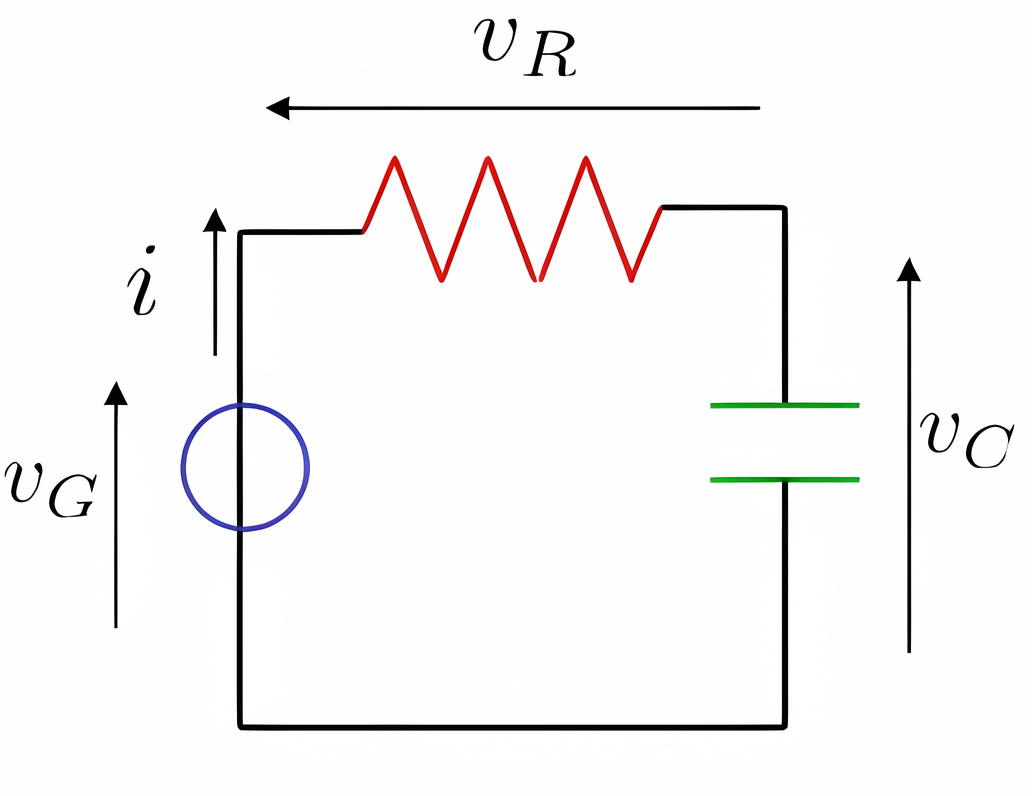
\includegraphics[scale=0.2]{Images/Es_cirucito_elettrico.png}
\end{center}
La legge che usiamo per definire il circuito (il nostro sistema) è la \textit{legge delle tensioni}
\[
    v_R (t) = v_G (t) - v_C(t)
\] 
le leggi del condensatore e del resistore sono 
\begin{align*}
    C \cdot  \dot v_C (t) &= i(t) & v_R (t) = R\cdot i(t)
\end{align*}
Scrivendo la formula in termini di $v_C (t)$ (“stato interno”) e $v_G (t)$ (“ingresso di controllo”)
\[
    \dot v_C (t) = \frac{1}{RC} \left(v_G (t) - v_C (t) \right)
\]




\section{Sistemi in forma di stato}
\subsection{Sistemi continui}
I \textit{sistemi continuti} sono sistemi in cui il tempo è una variabile reale: $t \in \mathbb{R}$
\begin{align*}
    \dot x(t) &= f \left( x(t), u(t), t \right) & &\text{equazione di stato}\\
    \dot y(t) &= h\left(x(t), u(t), t\right) & &\text{equazione  (trasformazione) di uscita }
\end{align*}
Definiamo inoltre $t_0$ come tempo iniziale e $x(t_0)=x_0$ come stato iniziale. \\
\textbf{N.B.} $\dot x(t) := \dfrac{d}{dt}x(t)$.
\vspace*{0.1cm}\\
Notazione:
\begin{itemize}
    \item $x(t) \in \mathbb{R}^n$ stato del sistema all'istante $t$
    \item $u(t) \in \mathbb{R}^m$ ingresso del sistema all'istante $t$
    \item $y(t) \in \mathbb{R}^p$ uscita del sistema all'istante $t$
\end{itemize}
\[
    x(t)=
    \begin{bmatrix}
        x_1(t)\\
        ...\\
        ...\\
        ...\\
        x_n(t)
    \end{bmatrix}
    \ \ \ \ \ 
    u(t) =
    \begin{bmatrix}
        u_1(t)\\
        ...\\
        ...\\
        ...\\
        u_m(t)
    \end{bmatrix}
    \ \ \ \ \ 
    y(t) = 
    \begin{bmatrix}
        y_1(t)\\
        ...\\
        ...\\
        ...\\
        y_p(t)
    \end{bmatrix}
\]
Da notare che $x(t)$ è un vettore mentre $x_1,...,x_n$ sono scalari.\\
$x(t)$ è una variabile interna che descrive il comportamento del sistema.


\subsubsection{Equazione di stato}
L'\textit{equazione di stato} è un'equazione ordinaria (ODE) vettoriale del primo ordine (cioè l'ordine massimo delle derivate è 1)
\begin{align*}
    \dot x_1(t) &= f_1 \left(x(t), u(t), t\right)\\
    &\dots\\
    \dot x_n (t) &= f_n \left(x(t), u(t), t\right)
\end{align*}
$\mathbb{R}^n$ è detto \underline{spazio di stato}, con $n$ ordine del sistema. La funzione di stato è $f: \mathbb{R}^n \times \mathbb{R}^m \times \mathbb{R} \rightarrow \mathbb{R}^n$.
\[
    \begin{bmatrix}
        \dot x_1(t)\\
        ...\\
        ...\\
        ...\\
        \dot x_n(t)
    \end{bmatrix} 
    =
    \begin{bmatrix}
        f_1\left(x(t),u(t),t\right)\\
        ...\\
        ...\\
        ...\\
        f_n\left(x(t),u(t),t\right)
    \end{bmatrix}
    := f\left(x(t),u(t),t\right)
\]
Avere solo derivate prime non è limitato, perché ad esempio posso inserire una prima variabile come derivata prima e una seconda variabile come derivata prima della prima variabile.

\subsubsection{Equazione di uscita}
L'equazione di uscita è un'equazione algebrica
\begin{align*}
    y_1(t) &= h_1 \left(x(t), u(t), t\right)\\
    &\dots\\
    y_p (t) &= h_p \left(x(t), u(t), t\right)
\end{align*}
$h : \mathbb{R}^n \times \mathbb{R}^m , \mathbb{R} \rightarrow R^p$ funzione di uscita
\[
    \begin{bmatrix}
        y_1(t)\\
        ...\\
        ...\\
        ...\\
        y_p(t)
    \end{bmatrix} 
    =
    \begin{bmatrix}
        h_1\left(x(t),u(t),t\right)\\
        ...\\
        ...\\
        ...\\
        h_p\left(x(t),u(t),t\right)
    \end{bmatrix}
    := h\left(x(t),u(t),t\right)
\]
\vspace*{0.2cm}
Se la soluzione $x(t)$ a partire da un istante iniziale $t_0$ è univocamente determinata da $x(t_0)$ e $u(\tau)$ con $\tau \geq t_0$, allora il sistema è detto \textbf{causale}, cioè lo stato dipende solo da ciò che accede in passato.\\
Sotto opportune ipotesi di regolarità della funzione $f$ si dimostra esistenza e unicità della soluzione dell'equazione (differenziale) di stato (Teorema di Cauchy-Lipschitz).



\subsection{Sistemi discreti}
Nei \textit{sistemi discreti} il tempo $t$ è una variabile intera, $t \in \mathbb{Z}$.
\begin{align*}
    x(t+1) &= f \left(x(t), u(t), t\right) & &\text{equazione di stato}\\
    y(t) &= h\left(x(t), u(t), t\right) & &\text{equazione (trasformazione) di uscita}
\end{align*}
L'equazione di stato è un'equazione alle differenze finite (FDE).
\vspace*{0.2cm}\\
Notazione:
\begin{itemize}
    \item $x(t) \in \mathbb{R}^n$ stato  del sistema all'istante $t$
    \item $u(t) \in \mathbb{R}^m$ ingresso del sistema all'istante $t$
    \item $y(t) \in \mathbb{R}^p$ uscita del sistema all'istante $t$
\end{itemize}
$x(t),u(t) \text{ e } y(t)$ sono uguali ai sistemi continui.\\
Per modellare sistemi discreti nel codice basta un ciclo {\fontfamily{lmtt}\selectfont for}.



\subsection{Esempio circuito elettrico}
Riprendiamo l'esempio del \hyperlink{Circuito elettrico}{circuito elettrico}; la formula trovata è 
\[
    \underbrace{\dot v_C(t)}_{\dot x(t)} = \frac{1}{RC} (\underbrace{v_G (t)}_{u(t)} - \underbrace{v_C (t)}_{x(t)} )
\]
In questo caso lo stato del sistema $x(t)$ è caratterizzato dalla variabile $v_C(t)$, l'ingresso dalla variabile $v_G(t)$. Supponiamo quindi di misurare (con un sensore) la tensione ai capi della resistenza, allora l'uscita del nostro sistema sarà $v_R(t)$
\begin{align*}
    \dot x(t) &= \frac{1}{RC} \left(u(t)-x(t)\right) &
    f(x,u) &= \frac{1}{RC}(u-x)
\end{align*}
da notare che in questo caso $f$ non è funzione del tempo.
\[
    v_R(t) = v_G(t) - v_C(t) \Longrightarrow y(t) = u(t) - x(t)
\]


\subsubsection{Esempio con parametri che variano nel tempo}
Supponiamo che la resistenza sia una funzione del tempo
\[
    R(t) = \overline{R} \left(1- \frac{1}{2} e^{-t} \right)
\]
allora 
\begin{align*}
    \dot x(t) &= \frac{1}{R(t)C} \left(u(t)-x(t)\right) &
    f(x,u,t) &= \frac{1}{R(t)C}(u-x)
\end{align*}
in questo caso $f$ è funzione del tempo.



\subsection{Esempio carrello}
\begin{center}
    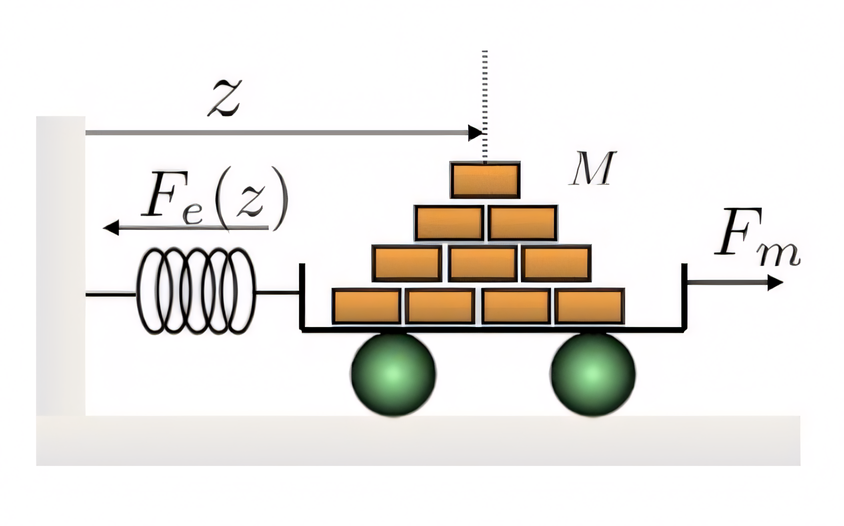
\includegraphics[scale=0.2]{Images/Es_carrello.png}
\end{center}
La legge che usiamo è la legge di Newton, prendendo $z$ come posizione del centro di massa
\[
    M \ddot  z = -F_e + F_m
\]
con $M$ massa e $F_e$ data da
\[
    F_e (z(t), t) = k(t)z(t)
\]
quindi la nostra equazione diventa
\[
    M \ddot  z(t) = -k(t)z(t) + F_m(t)
\]
Siccome nella nostra formula compare una derivata seconda di una variabile ci conviene definire lo stato del sistema con la variabile stessa e la derivata prima della variabile.\\
Definiamo quindi $x_1 := z$ e $x_2:=\dot z$, con stato $x := [x_1x_2]^T$, e $u := F_m$ (ingresso).
\vspace*{0.1cm}\\
Quindi possiamo scrivere, tenendo conto che $\dot x_2(t) = \ddot z$
\begin{align*}
    \dot x_1(t) &= x_2(t)\\
    \dot x_2(t) &= -\frac{k}{M} x_1(t) + \frac{u(t)}{M}
\end{align*}
\[
    f(x,u) = 
    \begin{bmatrix}
        f_1(x,u)\\
        f_2(x,u)
    \end{bmatrix}
    :=
    \begin{bmatrix}
        x_2\\
        -\dfrac{k}{M}x_1+\dfrac{u}{M}
    \end{bmatrix}
\]
Supponiamo di misurare $z(t)$ (sensore posizione), allora $y := z$
\begin{align*}
    \dot x_1(t) &= x_2(t)\\
    \dot x_2(t) &= -\frac{k}{M} x_1(t) + \frac{u(t)}{M}\\
    y(t) &= x_1(t)
\end{align*}
Sia $k(t) = k$ e, ricordando la formula dell'energia cinetica $E_{k}={\dfrac {1}{2}}mv^{2}$ e la formula dell'energia elastica $U={\dfrac {1}{2}}k\,\Delta x^{2}$, consideriamo come uscita l'energia totale $E_T (t) = \dfrac{1}{2} (k z^2 (t) + M \dot z^2 (t))$
\begin{align*}
    \dot x_1(t) &= x_2(t)\\
    \dot x_2(t) &= -\frac{k}{M} x_1(t) + \frac{u(t)}{M}\\
    y(t) &= \frac{1}{2} \left(k(t) x_1^2 (t) + M  x_2^2 (t)\right)
\end{align*}
quindi $h(x):= \dfrac{1}{2} (kx_1^2 + Mx_2^2)$.\\
\textbf{N.B.} Il risultato (l'uscita) vale, di solito, solo per il mio modello, in base a come l'ho impostato; nella realtà potrebbe essere diverso.


\subsection{Esempio auto in rettilineo}
\begin{center}
    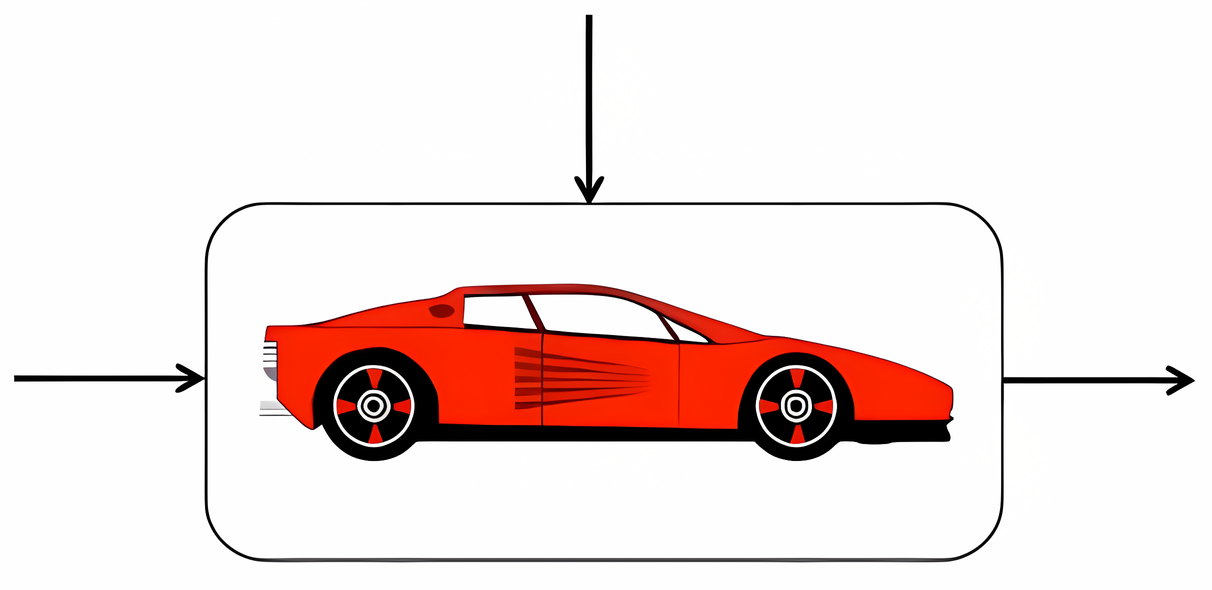
\includegraphics[scale=0.18]{Images/Es_Rettilineo.png}
\end{center}
Scriviamo la legge di Newton
\[
    M \ddot z = F_{\text{drag}} + F_m
\]
con $M$ massa e $F_{\text{drag}}$ data da
\[
    F_{\text{drag}} = -b \dot z
\]
Definiamo $x_1 := z$ e $x_2 := \dot z$ (stato $x := [x_1 x_2 ]^T$ ) e $u := F_m$ (ingresso). Supponiamo di misurare $z(t)$ (sensore posizione), allora $y := z$
\begin{align*}
    \dot x_1(t) &= x_2(t)\\
    \dot x_2(t) &= - \frac{b}{M} x_2(t) + \frac{1}{M}u(t)\\
    y(t) &= x_1(t)
\end{align*}
Proviamo a progettare un sistema per il \textit{cruise control}.\\
L'equazione della dinamica è
\[
    M \ddot z(t) = -b\dot z(t) + F_m (t)
\]
Siccome siamo interessati a controllare la velocità e non la posizione, allora consideriamo come stato solo la velocità: $x := \dot z$, $u := F_m$. Supponiamo di misurare $\dot z(t)$ (sensore velocità), allora $y := x$
\begin{align*}
    \dot x(t) &= - \frac{b}{M}x(t) + \frac{1}{M}u(t)\\
    y(t) &= x(t)
\end{align*}



\subsection{Esempio pendolo}
\begin{center}
    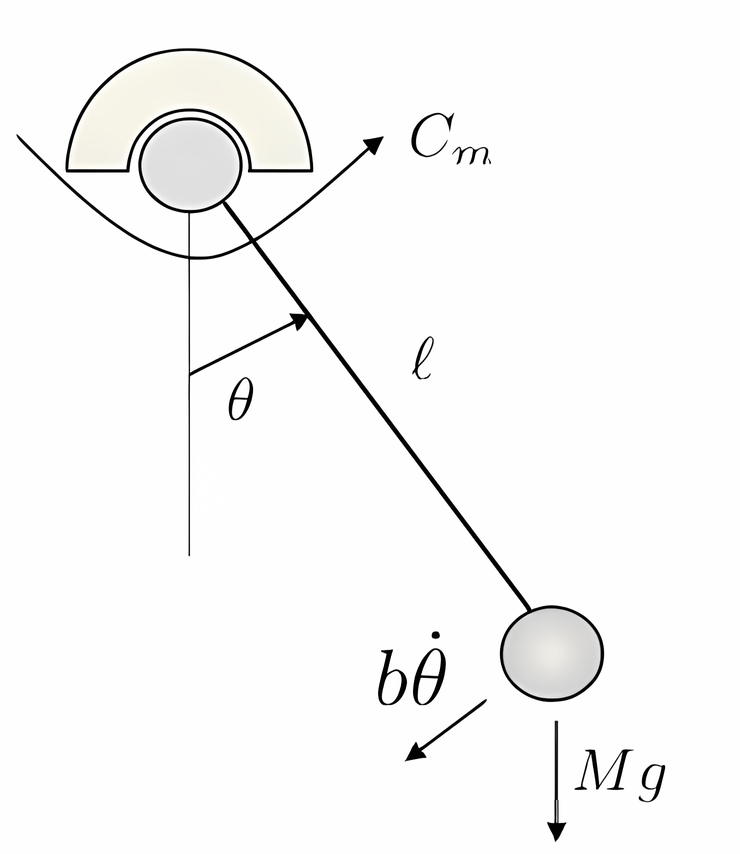
\includegraphics[scale=0.17]{Images/Es_pendolo.png}
\end{center}
Scriviamo l'equazione dei momenti
\[
    M \ell^2 \ddot \theta= C_{\T{grav}} + C_{\T{drag}} + C_m
\]
con $M$ massa e $C_{\T{grav}}$ e $C_{\T{drag}}$ date da
\begin{align*}
    C_{\T{grav}} &=M g \ell \sin(\theta) &
    C_{\T{drag}} &= -b \dot \theta
\end{align*}
con $b$ coefficiente d'attrito.
\vspace*{0.2cm}\\
Scriviamo l'equazione della dinamica, partendo dalla formula iniziale dei momenti

\[
    \ddot \theta(t) = -\frac{g}{\ell} \sin \left(\theta(t)\right) - \frac{b}{M \ell^2} \dot \theta(t) + \frac{1}{M \ell^2} C_m(t)
\]
Definiamo quindi $x_1 := \theta$ e $x_2 := \dot \theta$ (stato $x:= [x_1x_2]^T$) e $u := C_m$ (ingresso).\\
Supponiamo di misurare $\theta$ (sensore angolo) , allora $y := \theta$
\begin{align*}
    \dot x_1 (t) &= x_2(t)\\
    \dot x_2(t) &= -\frac{g}{\ell} \sin \left(x_1(t)\right) - \frac{b}{M \ell^2} x_2(t) + \frac{1}{M \ell^2} u(t)\\
    y(t) &= x_1(t)
\end{align*}
Se misuriamo invece la posizione verticale, allora $y := - \ell \cos(\theta)$ 
\begin{align*}
    \dot x_1 (t) &= x_2(t)\\
    \dot x_2(t) &= -\frac{g}{\ell} \sin \left(x_1(t)\right) - \frac{b}{M \ell^2} x_2(t) + \frac{1}{M \ell^2} u(t)\\
    y(t) &= - \ell \cos(\theta)
\end{align*}



\subsection{Traiettoria di un sistema}
Dato un istante iniziale $t_0$ e uno stato iniziale $x_{t_0}$, la funzione del tempo $(x(t), u(t)), \ t>t_0$, che soddisfa l'equazione di stato $\dot x(t) = f (x(t), u(t), t)$ si dice traiettoria (movimento) del sistema. In particolare, $x(t)$ si dice traiettoria dello stato. Consistentemente, $y(t)$ si dice traiettoria dell'uscita.
\vspace*{0.2cm}\\
\textbf{N.B.} per sistemi senza ingresso (quindi non forzati) la traiettoria dello stato $x(t), \ t>t_0$ è determinata solo dallo stato iniziale $x_{t_0}$.


\subsubsection{Esempio}
Definiamo un sistema con stato $x$ e stato iniziale $x_0$
\begin{align*}
    x &:=
    \begin{bmatrix}
        x_1\\
        x_2
    \end{bmatrix}
    &
    x_0 &:=
    \begin{bmatrix}
        5\\
        3
    \end{bmatrix}
    &
    t_0 &= 0
\end{align*}
\begin{align*}
    \dot x_1(t) &= x_2(t)\\
    \dot x_2(t) &= u(t)
\end{align*}
Assegno a $x_1$, $x_2$ e $u(t)$ le seguenti equazioni
\begin{align*}
    \overline{x_1}(t) &= 5+3t+t^2\\
    \overline{x_2}(t) &= 3+2t\\
    \overline{u}(t) &= 2
\end{align*}
Se le equazioni di $\overline{x_1}$ e $\overline{x_2}$ soddisfano le condizioni iniziali e la funzione di stato ($\dot x_1$ e $\dot x_2$) allora quelle equazioni sono la traiettoria del sistema.\\
Infatti
\[
    \overline{x_0} = 
    \begin{bmatrix}
        5+3t+t^2\\
        3+2t
    \end{bmatrix}_{t=0} 
    =
    \begin{bmatrix}
        5\\
        3
    \end{bmatrix}
\]
\begin{align*}
    &\overline{x_0} = 
    \begin{bmatrix}
        5+3t+t^2\\
        3+2t
    \end{bmatrix}_{t=0} 
    =
    \begin{bmatrix}
        5\\
        3
    \end{bmatrix}
    &
    \frac{d}{dt} 
    \begin{bmatrix}
        5+3t+t^2\\
        3+2t
    \end{bmatrix}
    =
    \begin{bmatrix}
        3+2t\\
        2
    \end{bmatrix}
\end{align*}



\subsection{Equilibrio di un sistema}
Dato un sistema (non forzato) $\dot x(t) = f (x(t), t)$, uno stato $x_e$ si dice \textit{equilibrio del sistema} se $x(t) = x_e$ , $t\geq t_0$ è una traiettoria del sistema.
\vspace*{0.2cm}\\
Dato un sistema (forzato) $\dot x(t) = f (x(t), u(t), t)$, $(x_e , u_e )$ si dice \textit{coppia di equilibrio} del sistema se $(x(t), u(t)) = (x_e , u_e )$, $t \geq t_0$ , è una traiettoria del sistema.
\vspace*{0.2cm}\\
Per un sistema (tempo invariante continuo) $\dot x(t) = f (x(t), u(t))$ data una coppia di equilibrio $(x_e,u_e)$ vale $f(x_e,u_e)=0$.\\
Se il sistema è non forzato, dato un equilibrio $x_e$ vale $f(x_e)=0$.


\subsubsection{Esempio pendolo}
\begin{align*}
    \dot x_1(t) &= x_2(t) &= f_1(x(t),u(t))\\
    \dot x_2(t) &= - \frac{G}{\ell} \sin (x_1(t)) - \frac{b}{M \ell ^2}x_2(t) + \frac{1}{M\ell^2}u(t) &=f_2(x(t),u(t))
\end{align*}
Siccome sappiamo che, data una coppia di equilibrio $(x_e,u_e)$, vale $f(x_e,u_e)=0$, allora per trovare l'equilibrio del pendolo imponiamo 
\[
    f(x_e,u_e)=0
\]
cioè:
\[
    \begin{cases}
        x_{2e}(t) = 0\\
        \\
        - \dfrac{G}{\ell} \sin (x_{1e}) - \dfrac{b x_{2e}}{M \ell ^2} + \dfrac{1}{M\ell^2}u_e =0
    \end{cases}
\]
sostituendo $x_{2e}(t)=0$ nell'ultima equazione
\[
    - \dfrac{G}{\ell} \sin (x_{1e}) + \dfrac{1}{M\ell^2}u_e =0 \Longrightarrow u_e = M G \ell \sin(x_{1e})
\]
In conclusione, le coppie di equilibrio del sistemo sono tutti fli $(x_{1e}, x_{2e},u_e)$ che soddisfano
\[
    \begin{cases}
        u_e = M G \ell \sin(x_{1e})\\
        x_{2e}=0
    \end{cases}
\]




\subsection{Classificazione dei sistemi in forma di stato}
La classe generale è  $x \in \mathbb{R}^n , u \in \mathbb{R}^m , y\in \mathbb{R}^p$
\begin{align*}
    \dot x(t) &= f (x(t), u(t), t) & &\T{equazione di stato}\\
    y(t) &= h(x(t), u(t), t) & &\T{equazione di uscita}  
\end{align*}
\begin{itemize}
    \item I sistemi \textbf{monovariabili} (SISO, Single Input Single Output) sono una sottoclasse di sistemi \textbf{multivariabili} (MIMO, Multiple Input Multiple Output); sono tali se $m=p=1$, altrimenti sono dei sistemi MIMO;
    \item I sistemi \textbf{strettamente propri} sono una sotto classe dei \textbf{sistemi propri}; sono tali se $y(t) = h(x(t),t))$, quindi se l'uscita dipende esclusivamente dall'ingresso, chiamati quindi sistemi causali (tutti i sistemi che abbiamo visto fin'ora sono sistemi propri).
    \item I sistemi \textbf{non forzati} sono una sotto classe dei \textbf{sistemi forzati}; un esempio di sistema non forzato è il seguente
    \begin{align*}
        \dot x(t) &= f(x(t),t)\\
        y(t) &= h(x(t),t)
    \end{align*}
    \item I sistemi \textbf{tempo invarianti} sono una sotto classe di sistemi \textbf{tempo  varianti}.\\
    I tempo invarianti sono tali se, data una traiettoria $ (x(t), u(t)), t\geq t_0$, con $x(t_0)=x_0$, per ogni $\Delta \in \mathbb{R}$ vale che $x(t_0+\Delta)=x_0$ allora $(x_{\Delta} (t), u_{\Delta} (t)) = (x(t-\Delta), u(t-\Delta))$ è una traiettoria.\\
    Si può dimostrare che sistemi tempo invarianti sono del tipo
    \begin{align*}
        \dot x(t) &= f (x(t), u(t)) &x(0)=x_0\\
        y(t) &= h(x(t), u(t))
    \end{align*}
    e senza senza perdita di generalità possiamo scegliere $t_0=0$.\\
    Graficamente:
    \begin{center}
        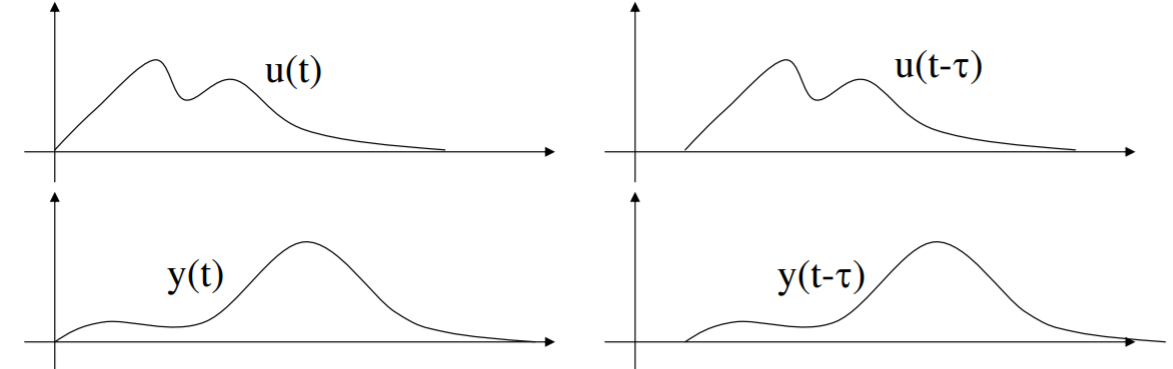
\includegraphics[scale=0.3]{Images/Sistemi_tempo_invarianti.png}
    \end{center}
    \item I \textbf{sistemi lineari} sono una sotto classe di \textbf{sistemi non lineari}.\\
    I sistemi lineari sono tali se le funzioni di stato e di uscita sono lineari in $x$ e $u$:
    \begin{align*}
        \dot x_1 (t) &= a_{11} (t)x_1 (t) + a_{12} (t)x_2 (t) + . . . + a_{1n} (t)x_n (t)+ b_{11} (t)u_1 (t) + b_{12} (t)u_2 (t) + . . . + b_{1m} (t)u_m (t)\\
        \dot x_2 (t) &= a_{21} (t)x_1 (t) + a_{22} (t)x_2 (t) + . . . + a_{2n} (t)x_n (t)+ b_{21} (t)u_1 (t) + b_{22} (t)u_2 (t) + . . . + b_{2m} (t)u_m (t)\\
        ...\\
        ...\\
        ...\\
        \dot x_n (t) &= a_{n1} (t)x_1 (t) + a_{n2} (t)x_2 (t) + . . . + a_{nn} (t)x_n (t)+ b_{n1} (t)u_1 (t) + b_{n2} (t)u_2 (t) + . . . + b_{nm} (t)u_m (t)
    \end{align*}
    per $y(t)$ invece 
    \begin{align*}
        y_1 (t) &= c_{11} (t)x1 (t) + c_{12} (t)x_2 (t) + . . . + c_{1n} (t)x_n (t)+ d_{11} (t)u_1 (t) + d_{12} (t)u_2 (t) + . . . + d_{1m} (t)u_m (t)\\
        y_2 (t) &= c_{21} (t)x_1 (t) + c_{22} (t)x_2 (t) + . . . + c_{2n} (t)x_n (t)+ d_{21} (t)u_1 (t) + d_{22} (t)u_2 (t) + . . . + d_{2m} (t)u_m (t)\\
        ...\\
        ...\\
        ...\\
        y_p (t) &= c_{p1} (t)x_1 (t) + c_{p2} (t)x_2 (t) + . . . + c_{pn} (t)x_n (t)+ d_{p1}(t)u_1 (t) + d_{p2} (t)u_2 (t) + . . . + d_{pm} (t)u_m (t)
    \end{align*}
\end{itemize}



\subsection{Proprietà dei sistemi lineari}
\subsubsection{Sistemi lineri in forma matriciale}
Definiamo le matrici $A(t) \in \mathbb{R}^{n \times n} , B(t) \in \mathbb{R}^{n \times m} , C(t) \in \mathbb{R}^{p \times n} , D(t) \in \mathbb{R}^{p \times m}$
\begin{align*}
    A(t) &= \begin{bmatrix}
        a_{11}(t) & ... & a_{1n}(t)\\
        .\\
        .\\
        a_{n1}(t) & ... & a_{nn}(t)
    \end{bmatrix}
    &
    B(t) &= \begin{bmatrix}
        b_{11}(t) & ... & b_{1m}(t)\\
        .\\
        .\\
        b_{n1}(t) & ... & b_{nm}(t)
    \end{bmatrix}\\
    C(t) &= \begin{bmatrix}
        c_{11}(t) & ... & c_{1n}(t)\\
        .\\
        .\\
        c_{p1}(t) & ... & c_{pn}(t)
    \end{bmatrix}
    &
    D(t) &= \begin{bmatrix}
        d_{11}(t) & ... & d_{1m}(t)\\
        .\\
        .\\
        d_{pn1}(t) & ... & d_{pm}(t)
    \end{bmatrix}
\end{align*}
quindi scriviamo
\[
    \begin{bmatrix}
        \dot x_1(t)\\
        .\\
        .\\
        \dot x_n(t)
    \end{bmatrix}
    = A(t)
    \begin{bmatrix}
        x_1(t)\\
        .\\
        .\\
        x_n(t)
    \end{bmatrix}
    + B(t)
    \begin{bmatrix}
        u_1(t)\\
        .\\
        .\\
        u_m(t)
    \end{bmatrix}
\]
che equivale a 
\begin{align*}
    \dot x(t) &= A(t) x(t) + B(t) u(t)\\
    y(t) &= C(t)x(t) + D(t) u(t)
\end{align*}


\subsubsection{Caso particolare: sistemi lineari tempo-invarianti}
\begin{align*}
    \dot x(t) = A x(t) + B u(t)\\
    y(t) = C x(t) + D u(t)
\end{align*}
con $A,B,C,D$ matrici costanti.


\subsubsection{Esempio carrello}
\begin{center}
    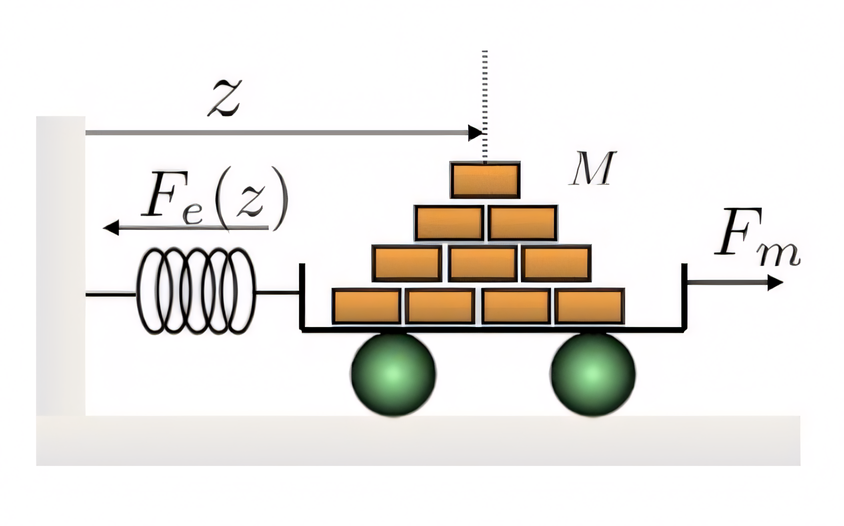
\includegraphics[scale=0.2]{Images/Es_carrello.png}
\end{center}
\begin{align*}
    \dot x_1(t) &= x_2(t)\\
    \dot x_2(t) &= - \frac{k(t)}{M}x_1(t) + \frac{1}{M} u(t)\\
    y(t) &= x_1(t)
\end{align*}

























\end{document}